% Chapter 5

\chapter{Pracovisko pre automatizovaný zber dát.}\label{Chapter5}
\lhead{Chapter 5. \emph{Pracovisko pre automatizovaný zber dát}}

Na popisovanom pracovisku možno automaticky merať vysokofrekvenčnú a
nízkofrekvenčnú kapacitu štruktúry MOS\@. Na obrázku~\ref{fig:5.1} je
zobrazené blokové zapojenie prístrojov, pomocou ktorých sú jednotlivé
metódy realizované.

\begin{figure}[h!]\centering
  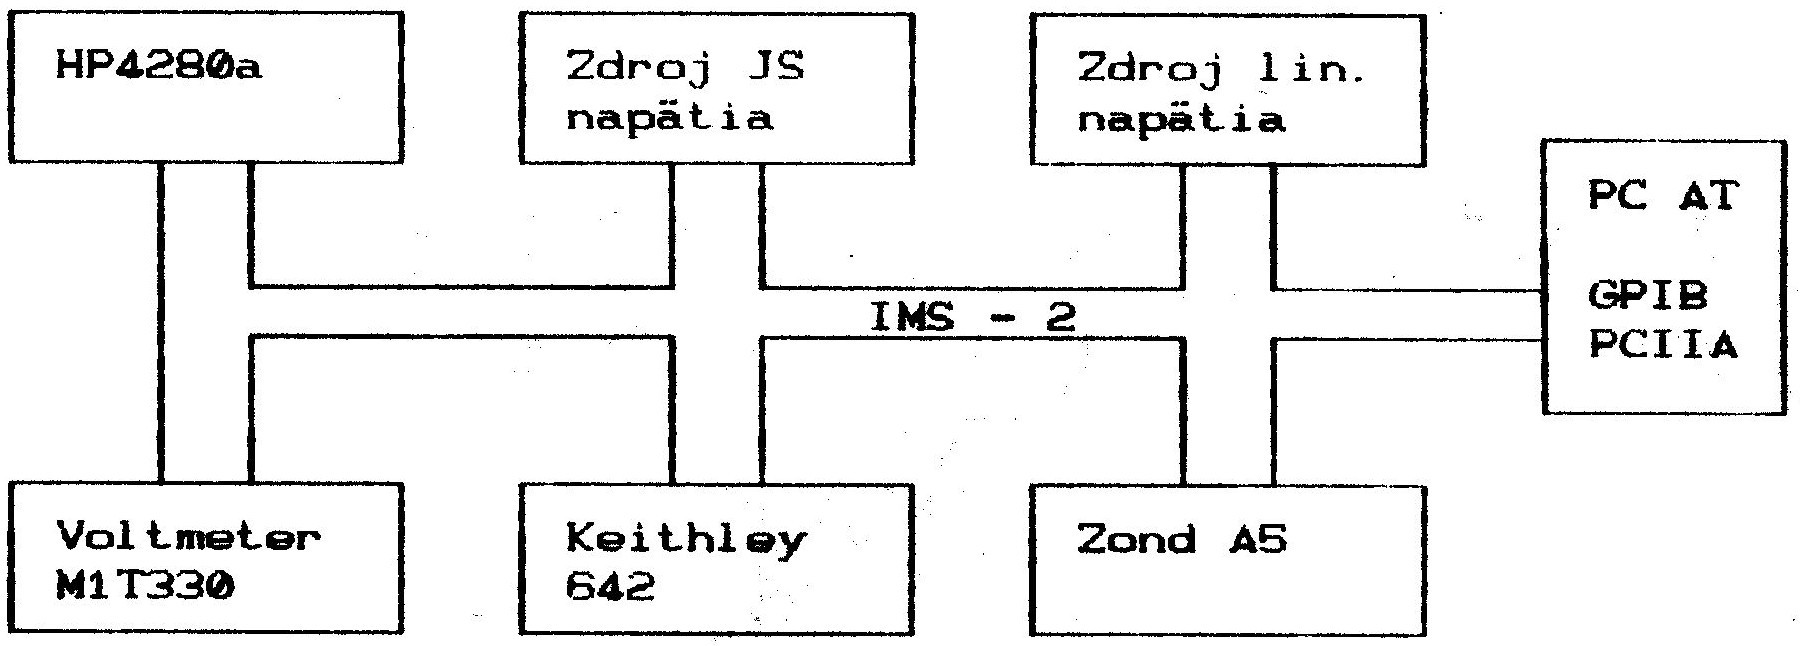
\includegraphics{Figures/fig-5-1.eps}% chktex-file 8
  \caption[Bloková schéma zapojenia prístrojov automatizovaného
    pracoviska]{Bloková schéma zapojenia prístrojov automatizovaného
    pracoviska pre určovanie plošného rozloženia parametrov štruktúr
    MOS s nehomogénnou dotáciou substrátu.}\label{fig:5.1}
\end{figure}

Riadiacim počítačom meraní je osobný počítač PC AT vybavený
interfejsom IMS-2 (norma IEEE 488) firmy National Instruments model
GPIB-PCIIA, ktorý pracuje ako riadič zbernice IMS-2. Všetky pripojené
prístroje sú vybavené interfejsom IMS-2, pomocou ktorého ich možno
diaľkovo ovládať a zberať namerané údaje. Okrem profesionálnych
meracích prístrojov HP4280a a Keithley 642 boli v experimente použité
zdroje jednosmerného napätia a zdroj lineárne narastajúceho napätia
postavené na Katedre mikroelektroniky. Voltmeter M1T330 je výrobkom
Metry Blansko a krokovacie hrotové zariadenie Zond A5 bolo dovezené zo
Sovietskeho Zväzu. Posledne spomínané zariadenie neobsahuje štandardne
interfejs IMS-2 a bolo dodatočne vybavené modulom IMS-2 vlastnej
konštrukcie~\cite{5.1}.

Ďalším novým prvkom našej realizácie pracoviska pre meranie štruktúr
MOS je možnosť automatického zberu dát po celej kremíkovej doske a ich
uloženie do diskového súboru pre následovné spracovanie. Programové
vybavenie pracoviska možno rozdeliť na programy (1) zberu dát (2)
spracovania dát (3) zobrazenia vysledkov a (4) pomocné
programy. Programy zberu dát umožňujú meranie C-V závislosti v
ľubovoľnom počte bodov kremíkovej dosky, ktorých pozície sú voliteľné
a sú definované operátorom.

Dôležitým momentom pri realizácii programov zberu dát bolo
zabezpečenie proti strate nameraných dát v dôsledku výskytu ľubovolnej
chyby (napr.\ výpadku napätia), alebo v prípade nutnosti prerušiť
meranie. Pretože trvanie zberu dát na kremíkovej doske s 300
štruktúrami sa pohybuje od 0.5 do 12 hodín v závislosti od
požadovaného druhu merania, bolo potrebné programovo zabezpečiť (1)
možnosť prerušenia merania operátorom v ľubovoľnom bode (2) možnosť
opätovného reštartovania zberu dát v bode, kde bol zber dát
prerušený. Zabezpečenie uchovania nameraných dát v prípade výskytu
chyby bolo realizované následovným spôsobom. Namerané dáta sú naraz
zapisované do diskového súboru vždy po ukončení merania na každej
štruktúre. Túto dátovu jednotku budeme v ďalsom označovat záznam. To
znamená, že k poškodeniu štruktúry dát môže prísť len v prípade
výskytu chyby v priebehu krátkeho časového úseku (rádove desiatky ms),
čím ale prichádza len k strate posledného záznamu. Pre tento prípad je
k dispozícii pomocný program, ktorý zkráti dátový súbor na požadované
množstvo záznamov, čím obnoví kompaktnosť súboru a umožní
reštartovanie zberu dát. Týmto spôsobom možno skrátiť dátovy súbor o
chybne namerané dáta aj po prerušení zberu dát operátorom, ak bola
zistená nejaká závada v priebehu merania. Zároveň je k dispozícii
pomocný program, ktorý umožňuje prepísanie ľubovolného počtu záznamov
dátového súboru. Užitočnosť tohto programu vysvetlíme v následovnom
príklade.

Predstavme si, že v priebehu zberu dát došlo (napr.dôsledkom vplyvov
okolia) ku chybe, ktorá trvala krátky časový úsek, čo spôsobilo, že
časť záznamov dátového súboru obsahuje chybné dáta. Príkladom môže byť
nedokonalosť kontaktu hrotu s meranou vzorkou spôsobená vibráciami. To
sa často zistí až pri vyhodnocovaní merania, prípadne pri zobrazení
výsledkov. Po určení pozícií štruktúr na testovanej kremíkovej doske,
v ktorých sme namerali chybné údaje, môžeme v týchto bodoch meranie
zopakovať a pomocným programom prepísať záznamy v pôvodnom dátovom
súbore.

Uvedeným spôsobom boli realizované programy zberu dát pre HF C-V,
kvázistaticku C-V metódu, meranie kapacity oxidovej vrstvy a metódu
konštantnej šírky oblasti priestorového náboja. Takto sme ale nemohli
automatizovať Q-C metódu, pretože použitý interfejs prístroja Keithley
642 neumožňuje diaľkové ovládanie skratovania vstupných svoriek
meracieho prístroja, čím nemožno automatizovať vynulovanie náboja v
spoločnom bode zapojenia kondenzátorov, ktorý sa tam dostane vplyvom
zvodových prúdov.

Pre pohodlnú manipuláciu s dátovými súbormi bola zvolená následovná
koncepcia pomenovania dátovych súborov. Pomenovanie súboru v operačnom
systéme MS DOS pozostáva z mena súboru a prípony.  Meno súboru
predstavuje v našom prípade názov meranej kremíkovej dosky a prípona
označuje druh dát, ktoré súbor obsahuje. Principiálne možno rozdeliť
uvedené dátove súbory na dva typy podľa dát, ktoré obsahujú jednotlivé
záznamy. Môže to byť funkčná závislosť alebo parameter. Ak sa jedná o
funkčnú závislosť, potom prvý záznam v dátovom súbore obsahuje počet
bodov, v ktorých bola funkčná závislosť zosnímaná a hodnoty nezávislej
premennej. Ďalšie záznamy obsahujú pozíciu štruktúry na kremíkovej
doske, vyjadrenú dvoma celými číslami (X,Y), počet bodov a funkčné
hodnoty.  Opakujúca sa informácia o počte bodov funkčnej závislosti
nie je redundantná, pretože v prípade neúspešnosti merania
(napr.prieraz) na štruktúre (X,Y) obsahuje číslo -1, ktoré oznamuje
neprítomnosť funkčných hodnôt v zázname. Príkladom môže byť HF C-V
závislosť. Prvý záznam obsahuje počet meraní kapacity na jednej
štruktúre a hodnoty napätia hradla. Ďalšie záznamy obsahujú pozíciu
štruktúry (X,Y), počet bodov a hodnoty kapacity zodpovedajúce
hradlovým napätiam z prvého záznamu. Súbory druhého typu pozostávajú
len zo záznamov, ktoré obsahujú pozície štruktúry (X,Y) a hodnotu
parametra. Ako príklad uvedieme dátový súbor, ktorý obsahuje kapacity
oxidovej vrstvy štruktúr MOS\@. Pretože sa jedná o rozsiahle dátové
súbory bola zvolená binárna forma záznamu.  Celočíselné hodnoty majú
dĺžku 2 bajty a čísla s pohyblivou desatinnou čiarkou zaberajú 4
bajty.

Pre prípad, že by bol potrebný dátovy súbor, obsahujúci dáta vo forme
ASCII, je k dispozícii pomocný program, ktorý po zadaní pozície
štruktúry (X,Y) vytvorí tento dátový súbor a zapíše do neho dáta,
ktoré obsahuje záznam s pozíciou (X,Y). Ak sa jedná o funkčnú
závislosť, zapíše do výstupného súboru vo forme ASCII aj hodnoty
nezávislej premennej.

\section{Meranie HF C-V závislostí.}\label{sec:5.1}

HF C-V závislosť štruktúry MOS meriame pomocou prístroja HP4280a,
ktorý určuje zároveň kapacitu a vodivosť meranej vzorky na základe
fázového posunu madzi HF napäťovým signálom (1MHz,30mV) a meraným
prúdom. Prístroj HP4280a je vybavený vlastným procesorom, ktorý riadi
jeho vnútorné funkcie a operátorovi poskytuje komfortné ovládanie. Pre
meranie HF C-V závislosti musíme nastaviť požadovaný interval napätia,
v ktorom sa má merať kapacita (Vstart, Vstop) a napäťový krok Vstep,
ktorým sa bude jednosmerné napätie meniť. Časové pomery merania sa
určujú ďalšími dvoma parametrami. Thold určuje čas, počas ktorého bude
na meranej vzorke pripojené napätie Vstart pred začiatkom
merania. Tento čas je potrebný na ustálenie prechodových javov, v
prípade že ich nechceme merať. Parameter Tdelay určuje dobu pozdržania
merania po vykonaní napäťového kroku.

Pre automatizované meranie štruktúr sme zvolili najvýkonnejší mód
prístroja HP4280a, v ktorom podľa vopred nastavených parametrov
automaticky vykoná celé meranie a namerané dáta uloží do vnútornej
pamäte.  Prenos dát z prístroja HP4280a do riadiaceho počítača sa
vykoná v binárnej forme, čím nestrácame čas konverziou medzi binárnou
formou a formou ASCII a zároveň binárna forma predstavuje menšie
množstvo prenášaných bajtov. Ukončenie merania a pripravenosť na
prenos dát signalizuje prístroj HP4280a nastavením signálu SRQ
(Service Request) na zbernici IMS-2, čím je synchronizovaná jeho
činnosť s riadiacim počítačom.  Tu možno spomenúť užitočnú vlastnosť
interfejsu GPIB-PCIIA~\cite{5.2}, ktorý po detekovaní signálu SRQ môže
automaticky vykonať sériové hlásenie prístrojov (Serial Poll) a po
nájdení prístroja, ktorý žiada o obsluhu uložiť jeho stavové slovo do
internej pamäte. Tým je vodič SRQ zbernice IMS-2 uvolnený a interfejs
GPIB-PCIIA môže reagovať na žiadosť o obsluhu od ďalších
prístrojov. Ak riadiaci program požaduje stavové slovo prístroja,
ktorý žiadal o obsluhu, interfejs GPIB-PCIIA ho vydá zo svojej
internej pamäte.

Použitím automatického riadenia merania a binárneho prenosu dát sa
podarilo dosiahnuť minimálny čas HF C-V merania.  Konkrétne hodnoty
trvania meraní a časové diagramy sú v časti~\ref{sec:5.4}.

Ak potrebujeme určiť koncentračný profil dotujúcich prímesí vo väčšej
hĺbke, ako je šírka OPN v stave inverzie, musime zmerat C-V závislosť
v stave hlbokého ochudobnenia. V tomto prípade sa vždy po napäťovom
skoku do stavu hlbokého ochudobnenia (a zmerania kapacity) musíme
vrátiť na určitý čas do stavu akumulácie. Prístroj HP4280a nemá mód
činnosti, ktorý by automaticky riadil tento druh merania. Preto musíme
každé meranie kapacity riadiť samostatne. Merací cyklus riadiaceho
programu potom obsahuje nastavenie požadovaného hradlového napätia,
prevedenie merania kapacity (spustenie merania a čakanie na jeho
ukončenie) a prenos dát z meracieho prístroja do riadiaceho počítača,
pričom všetky uvedené prenosy sa vykonávajú vo forme ASCII\@. Oproti
štandardnej HF C-V metóde sa dĺžka merania jedného bodu C-V závislosti
o rád zväčší.

Presnosť určenia koncentračného profilu dotujúcich prímesí silne
závisí od presnosti určenia kapacity oxidovej vrstvy.  Preto je
kapacita oxidu určovaná pomocou samostatného programu, ktorý meria
kapacitu štruktúry MOS pre zadané hradlové napätie ďaleko v akumulácii
a namerané hodnoty uloží do samostatného dátového súboru.

\section{Meranie kvázistatických C-V závislostí.}\label{sec:5.2}

Kvázistatickú C-V závislosť štruktúry MOS meriame pomocou zdroja
lineárne narastajúceho napätia, elektromera Keithley 642 a voltmetra
M1T330. Kapacitu štruktúry MOS určíme zo vzťahu

\begin{equation}\label{eq:5.1}
  C_{mos}^{LF} = i\ {\bigg[\frac{dV_{g}}{dt}\bigg]}^{-1}
\end{equation}

Presné meranie nabíjacieho prúdu štruktúry MOS je hlavným problémom
kvázistatickej C-V metódy. Firma Keithley dodáva k svojmu meraciemu
prístroju viac druhov interfejsov IMS-2. V našej meracej zostave je
použitý model 1793/6423, ktorý okrem prenosu nameraných dát neplní
žiadne ďalšie funkcie a činnosť prístroja musíme ovládať manuálne z
predného panelu.  Pred začiatkom merania je potrebné nastaviť meranú
veličinu (okrem prúdu možno merať ešte napätie a náboj) a merací
rozsah prístroja.

Meranie a prenos dát z elektrometra do riadiaceho počítača môže
prebiehať v dvoch módoch, ktoré sa odlišujú adresou
prístroja~\cite{5.3}. V kontinuálnom móde pracuje A/D prevodník
prístroja nepretržite a na žiadosť o vyslanie dát do počítača
interfejs vyšle posledné ukončené meranie (v tomto momente už môže byť
začatý ďalší A/D prevod). V spúšťanom móde A/D prevodník čaká na povel
k začatiu merania z interfejsu, ktorý dostane po žiadosti riadiaceho
počítača o vyslanie nameraných dát. Potom prebehne A/D prevod a
namerané dáta sú odoslané do počítača. Doba merania prístroja Keithley
642 je 400 ms. Táto doba je potrebná na ustálenie dynamických javov,
ktoré spôsobuje komunikácia po zbernici IMS- 2. Pretože interfejs
prístroja nie je galvanicky oddelený od meracej časti, majú obvod
merania prúdu a zbernica IMS-2 spoločnú zem. Tým komunikácia zbernice
IMS-2 počas A/D prevodu spôsobuje zašumenie meraného signálu.  Tento
problém možno odstrániť použitím spúšťaného módu, v ktorom pristroj po
prijatí žiadosti o vyslanie nameraných dát najprv počká na ustálenie
dynamických javov a potom vykoná A/D prevod.

Okrem prúdu potrebujeme pre výpočet kapacity poznať rýchlosť nárastu
napätia na hradle štruktúry MOS, ktorú určíme následovným spôsobom.
Meranie vykonáme vo vačšom napäťovom intervale, ako je požadované. V
štartovacom a koncovom úseku (mimo požadovaného intervalu napätí)
odmeriame hodnoty lineárne narastajúceho napätia hradla a zároveň
zmeriame čas pre každú hodnotu napätia. Čas meriame vnútornými
hodinami riadiaceho počítača s rozlíšením 1/12 s. Lineárnou regresiou
spomemutých dát určíme smernicu závislosti $V_{g}(t)$, ktorú použijeme
pri výpočte kapacity.

Ako sme už spomenuli meranie prúdu trvá 400 ms.  V snahe získať čo
najviac meraných bodov C-V závislosti sme zvolili následovný postup na
určenie napätia hradla zodpovedajúce meranému prúdu. Súčasne s meraním
prúdu odčítame čas, ktorý uplynul od začiatku merania a napätie hradla
vypočítame pomocou smernice závislosti $V_{g}(t)$. Odčítanie a
uloženie uplynutého času je rýchla operácia riadiaceho počítača, čím
získame čas, ktorý by sme stratili meraním napätia pomocou
voltmetra. Ďalšou výhodou uvedeného postupu je, že dostávame vyhladené
hodnoty priebehu napätia hradla v čase. V prípade, že by sme merali
priamo prúd aj napätie, dostali by sme chybami merania zaťažené tak
funkčné hodnoty ako aj hodnoty nezávislej premennej, čo by mohlo
prinášať problémy pri vyhladzovaní nameraných dát.

Napriek tomu, že meranie prúdu a času prebieha automaticky v meracej
slučke, nemusíme vždy získat C-V závislosť s ekvidištantným krokom v
napäťovej ose a zároveň nemôžeme dopredu určiť pri akom hradlovom
napätí odmeriame kapacitu.  Predspracovanie nameraných dát pred
zápisom do diskového súboru preto pozostáva z aproximácie C-V
závislosti pomocou kubických splajn-funkcií a výpočte kapacity
štruktúry MOS pre zadané hodnoty napätia. Je potrebné voliť hodnoty
napätia hradla v súlade s HF C-V meraním, čo uľahčí výpočet tých
parametrov štruktúr MOS, ktore sa určujú z HF a kvázistatickej C-V
závislosti.

Dá sa ukázať~\cite{5.4}, že kubické splajn-funkcie vznikajú
minimalizáciou kvadratického funkcionálu

$\int_{a}^{b}{(y^{''}(x))}^{2}dx$

ktorý je analógom energie ohybu pružného nosníku. Ak doplníme
podmienku minimalizácie uvedeného funkcionálu podmienkou najmenších
štvorcov vzdialenosti aproximačných funkcií a nameraných bodov,
vznikne aproximácia pomocou kubických splajn-funkcií. V našom programe
sme použili dvojicu podprogramov z numerickej knižnice NAG (Numerical
Algorythm Group), ktorých označenie je E02BAF a E02BCF\@. Podprogram
E02BAF na základe zadaných bodov vypočíta koeficienty aproximačných
B-splajn polynómov.  Užívateľovi je daná možnosť zvoliť uzly, medzi
ktorými sa nachádzajú jednotlivé B-splajn polynómy. Numerická metóda
tvorby koeficientov je stabilná dokonca aj pre viacnásobné
(tzn.koincidenčné) uzly~\cite{5.5, 5.6} (citované v príručke NAG). Z
teórie splajnových funkcií potom vyplýva, že pomocou viacnásobných
uzlov môžeme aproximovať funkcie s nespojitými deriváciami. Túto
vlastnosť sme použili pri aproximácii kvázistatickej C-V závislosti,
ktorá môže vykazovať nespojitosť derivácií v bode začiatku slabej
inverzie. Pri prechode medzi ochudobnením a stavom slabej inverzie tu
dochádza vplyvom exponenciálnej závislosti koncentrácie minoritných
nosičov od elektrického potenciálu k prudkej zmene kapacity. Do tohto
bodu sme umiestnili tri koincidenčné uzly, čím sme umožnili
nespojitosť derivácii 1., 2.\ a 3.\ rádu. Následne vypočítané hodnoty
kapacity pomocou podprogramu E02BCF vykazujú dobré aproximačné
vlastnosti. Uvedeným postupom sme odstránili prekmity aproximačných
polynómov, ktoré často vznikajú pri aproximácii funkcií s väčšou
zmenou gradientu.

\section{Meranie metódou konštantnej šírky OPN.}\label{sec:5.3}

Pre meranie metódou konštantnej šírky OPN sme použili prístroje
HP4280a a zdroj jednosmerného (JS) napäťia, ktorý bol postavený na
Katedre mikroelektroniky. Merací obvod prístroja HP4280a pozostáva z
vnútorného zdroja JS napätia (INT BIAS), zdroja HF signálu a
ampérmetra (označeného A)~\cite{5.7}. Vnútorný zdroj JS napätia má
rozsah $(-100.0,+100.0)V$ s rozlíšením $0.1V$, avšak v rozsahu
$(-2.0,+2.0)V$ môžeme nastavovať napätie s rozlíšením $0.001V$. Ak
meriame štruktúry MOS vytvorené na kvalitných kremíkových substrátoch,
relaxácia nerovnovážnych nosičov náboja prebieha pomaly, čo spôsobuje
aj pomalú zmenu kapacity štruktúry MOS\@. Aby sme mohli udržiavať
konštantnú veľkosť nerovnovážnej kapacity štruktúry MOS potrebujeme
meniť hradlové napätie podľa možnosti s čo najmenšími zmenami. Pre
tento účel je vhodný napäťový rozsah (-2.0,+2.0) V vnútorného JS
zdroja prístroja HP4280a. Pre uvedenie štruktúry MOS do nerovnovážneho
stavu hlbokého ochudobnenia použijeme externý zdroj JS napätia, ktorý
môže nastavovať napätie v intervale (-40.0, +40.0) V s rozlíšením 0.1
V. Prístroj HP4280a umožňuje veľkú flexibilitu konfigurácie elementov
meracieho obvodu. K dispozícii je 14 módov. Pre náš experiment sme
zvolili mod 11~\cite{5.2}, ktorý umožňuje pripojenie externého zdroja
JS napätia.

\begin{figure}[h!]\centering
  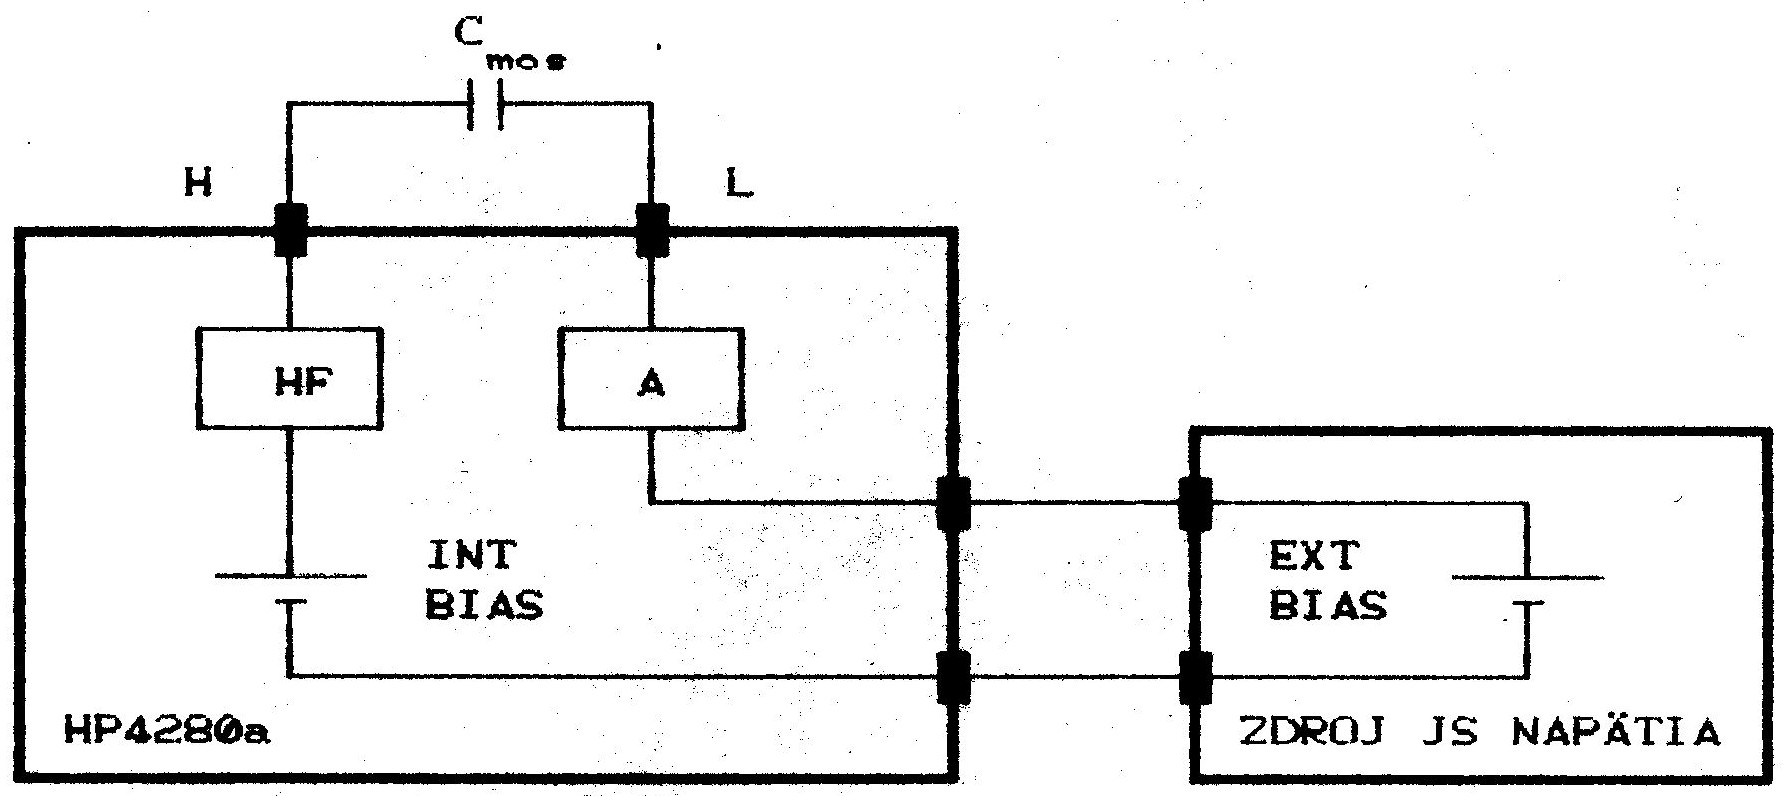
\includegraphics{Figures/fig-5-2.eps}
  \caption[Zapojenie prístrojov pre metódu konštantnej šírky
    OPN]{Zapojenie prístrojov pre metódu konštantnej šírky
    OPN.}\label{fig:5.2}
\end{figure}

Meranie zavislosti $V_{g}(t)$ potom prebieha v následovných
krokoch. Pomocou externého zdroja JS napätia privedieme štruktúru MOS
do nerovnovážneho stavu. Zo zmeny kapacity $\Delta{C}$, ktorú
odmeriame prístrojom HP4280a, vypočítame pomocou vzťahu~\ref{eq:3.9}
požadovanú zmenu napätia hradla $\Delta{V_{g}}$. Ak je jej veľkosť v
absolútnej hodnote väčšia ako $0.001 V$ zmeníme hodnotu napätia hradla
o $\Delta{V_{g}}$, čím udržiavame konštantnú hodnotu nerovnovážnej
kapacity štruktúry MOS\@. Pri každej zmene napätia hradla odčítame
čas, kedy táto zmena nastala. Meranie závislosti $V_{g}(t)$ ukončíme,
ak uplynul čas merania (označme ho $T_{hold}$), ktorý zadáva operátor,
prípadne ak zmena hradlového napätia presiahla hraničné hodnoty
intervalu $(-2.0,+2.0) V$.  Experimentálne sa ukázalo, že programová
spätnoväzobná slučka zabezpečujúca konštantnú hodnotu kapacity pracuje
dostatočne rýchlo a presne. Počas prevádzaných experimentov bolo
kolísanie udržiavanej kapacity lepšie ako 1\%.

Meranie opakujeme pre rôzne hodnoty kapacity štruktúry MOS v
nerovnovážnom stave, aby sme mohli určiť generačnú dobu minoritných
nosičov náboja podľa vzťahu~\ref{eq:3.10}.

Parametrami riadiaceho programu je interval, v ktorom sa má pohybovať
hranica OPN $(W_{start}, W_{stop})$ s krokom $W_{step}$. Ďalším
parametrom je hodnota $T_{hold}$, ktorá udáva maximálnu dobu merania
jednej závislosti $V_{g}(t)$.

Riadiaci program vyžaduje pre svoju činnosť dátové súbory s nameranými
C-V závislosťami hlbokého ochudobnenia a kapacitami oxidovej vrstvy
testovaných štruktúr kremíkovej dosky. Pomocou týchto vopred
nameraných dát a zo zadanej vzdialenosti hranice OPN potom určuje
počiatočné hradlové napätie pre nastavenie externého zdroja JS
napätia.  Pre svoju činnosť potrebuje riadiaci program ešte jeden
dátovy súbor, obsahujúci koncentračné profily dotujúcich prímesí
meraných štruktúr MOSň2. Hodnoty koncentrácie sú potrebné pri
vyčíslovaní zmeny napätia hradla štruktúry MOS podľa
vzťahu~\ref{eq:3.9}.

Po zmeraní závislosti $V_{g}(t)$ určíme lineárnou regresiou jej
smernicu. Z uskutočnených experimentov sa ukazuje, že minimálna doba
merania zavislosti $V_{g}(t)$, kedy ešte možno očakávať akceptovateľné
výsledky je pre substráty s hodnotami $\tau_g$ rádove $10^{3}\mu{s}$
približne $T_{hold}=10s$. Počas tejto doby prichádzalo k zmene napätia
hradla v rozsahu $50-500 mV$ v závislosti od šírky OPN a v závislosti
od prírastku minoritných nosičov z oblasti mimo OPN\@. Zároveň bolo z
grafického znázornenia závislosti $\frac{dV_g}{dt}=f(w)$ vidieť vplyv
prírastku minoritných nosičov náboja z oblasti mimo OPN, čo sa
prejavilo približne rovnakým sklonom závislostí
$\frac{dV_g}{dt}=f(w)$, ale rôznou absolútnou hodnotou. Zo zobrazenia
závislostí $\frac{dV_g}{dt}=f(w)$ na celej kremíkovej doske vyplýva,
že akceptovateľné hodnoty $\tau_{g}$ možno počítať jedine z derivácie
funkcie $\frac{dV_g}{dt}=f(w)$ podľa w (vzťah~\ref{eq:3.10}
príp.~\ref{eq:3.7}) a v žiadnom prípade nie z jej fukčných hodnôt
(vzťah~\ref{eq:3.5}). Do výstupného dátového súboru sme ukladali
funkčné závislosti $\frac{dV_g}{dt}=f(w)$.

Z princípu metódy vyplýva minimálna vzdialenosť od povrchu polovodiča,
v ktorej je možno určovať $\tau_{g}$. Touto hranicou je šírka OPN
zodpovedajúca počiatku slabej inverzie v polovodiči.

\section{Časové diagramy použitých metód.}\label{sec:5.4}

Aby sme mohli odhadnúť dobu merania pre jednotlivé metódy, znázorníme
graficky časové závislosti hradlového napätia štruktúry MOS\@. Okrem
rovnovážnej HF C-V metódy, kde je celý priebeh merania riadený
procesorom prístroja HP4280a a jeho časový diagram je prevzatý z
manuálu~\cite{5.7}, boli časové diagramy určené na základe
experimentálne nameraných hodnôt. Tieto časové hodnoty sú závislé od
druhu riadiaceho počítača a od optimalizácie riadiacich programov. V
našom experimente sme použili osobný počítač PC AT, pracujúci na
frekvencii 10 MHz s koprocesorom 80287 (6 MHz) a pevným diskom s dobou
prístupu 28 ms. Riadiace programy boli kompilované bez optimalizácie
na rýchlosť s použitím emulačnej knižnice podprogramov pre matematické
operácie s plávajúcou čiarkou.

V spojení s časovými diagramami uvedieme aj rozsahy napätí použitých
prístrojov.

\par\emph{POZNÁMKA.} V prípade, ak je pri maximálnej hodnote časového
údaju uvedený údaj `neohraničené', znamená to, že jeho maximálna
veľkosť závisí od dátového typu zodpovedajúcej premennej riadiaceho
programu, prípadne od rozsahu prístroja.


\newpage
\subsection{Rovnovážna HF C-V závislosť.}\label{sec:5.4.1}

\begin{figure}[h!]\centering
  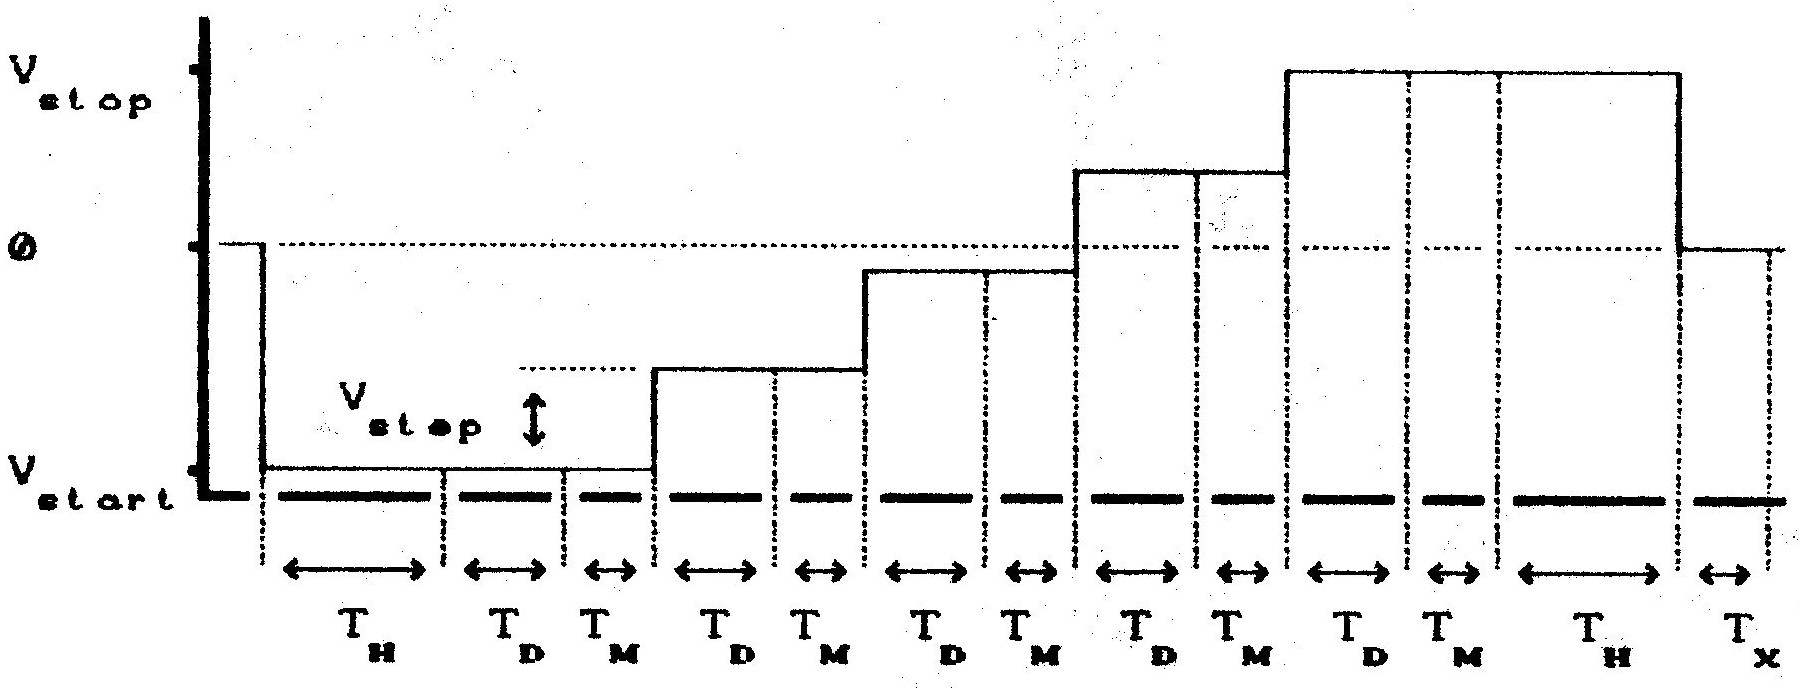
\includegraphics{Figures/fig-5-3.eps}
  \caption[Časový diagram rovnovážnej HF C-V metódy]{Časový diagram
    rovnovážnej HF C-V metódy.}\label{fig:5.3}
\end{figure}

\begin{table}[h!]\centering
  \begin{tabular}{l p{0.5\linewidth} l l}
    param.      & popis parametra & min. & max.hodnota\\
    \hline% chktex-file 44
    $T_H$       & čas ustálenia \dotfill & $3 ms$ &  $650 s$\\
    $T_D$       & čas pozdržania merania \dotfill & $3 ms$ & $650 s$\\
    $T_M$       & čas merania \dotfill & $40 ms$\\
    $T_X$       & binárny prenos dát,\\
                & predspracovanie dát,\\
                & uloženie dát do súboru,\\
                & posuv stolíka na ďalšiu štruktúru \dotfill & $\sim 7 s$\\
    $V_{start}$ & \dotfill & $-100.0 V$ & $+100.0 V$\\
    $V_{stop}$  & \dotfill & $-100.0 V$ & $+100.0 V$\\
    $V_{step}$  & \dotfill & $\pm 0.001 V$ & $\pm 200.0 V$\\
    \hline
  \end{tabular}
  \caption[Časový diagram rovnovážnej HF C-V metódy]{Časový diagram
    rovnovážnej HF C-V metódy.}\label{tab:5.1}
\end{table}

\newpage
\subsection{Nerovnovážna HF C-V závislosť.}\label{sec:5.4.2}

\begin{figure}[h!]\centering
  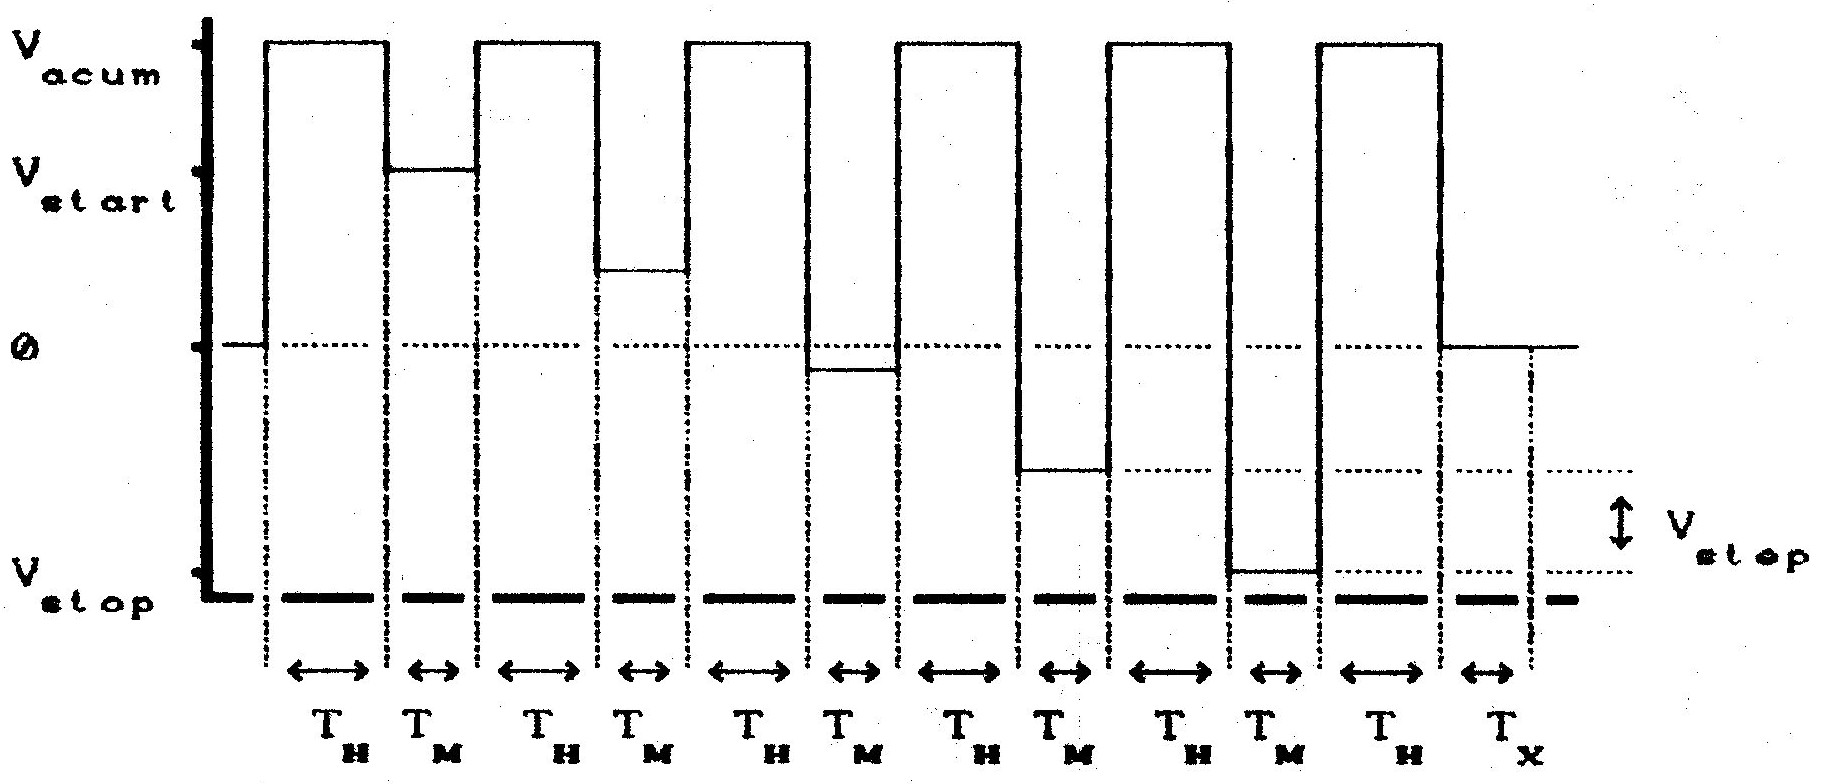
\includegraphics{Figures/fig-5-4.eps}
  \caption[Časový diagram nerovnovážnej HF C-V metódy]{Časový diagram
    nerovnovážnej HF C-V metódy.}\label{fig:5.4}
\end{figure}

\begin{table}[h!]\centering
  \begin{tabular}{l p{0.5\linewidth} l l}
    param.      & popis parametra & min. & max.hodnota\\
    \hline
    $T_H$       & čas relaxácie minoritných nosičov náboja \dotfill & $0 s$ &  neohraničené\\
    $T_M$       & čas merania a prenos dát \dotfill & $330 ms$\\
    $T_X$       & predspracovanie dát,\\
                & uloženie dát do súboru,\\
                & posuv stolíka na ďalšiu štruktúru \dotfill & $\sim 4s$\\
    $V_{start}$ & \dotfill & $-100.0$ & $+100.0 V$\\
    $V_{stop}$  & \dotfill & $-100.0$ & $+100.0 V$\\
    $V_{step}$  & \dotfill & $\pm 0.001$ & $\pm 200.0 V$\\
    $V_{acum}$  & \dotfill & $-100.0$ & $+100.0 V$\\
    \hline
  \end{tabular}
  \caption[Časový diagram nerovnovážnej HF C-V metódy]{Časový diagram
    nerovnovážnej HF C-V metódy.}\label{tab:5.2}
\end{table}

\newpage
\subsection{Kvázistatická C-V závislosť.}\label{sec:5.4.3}

\begin{figure}[h!]\centering
  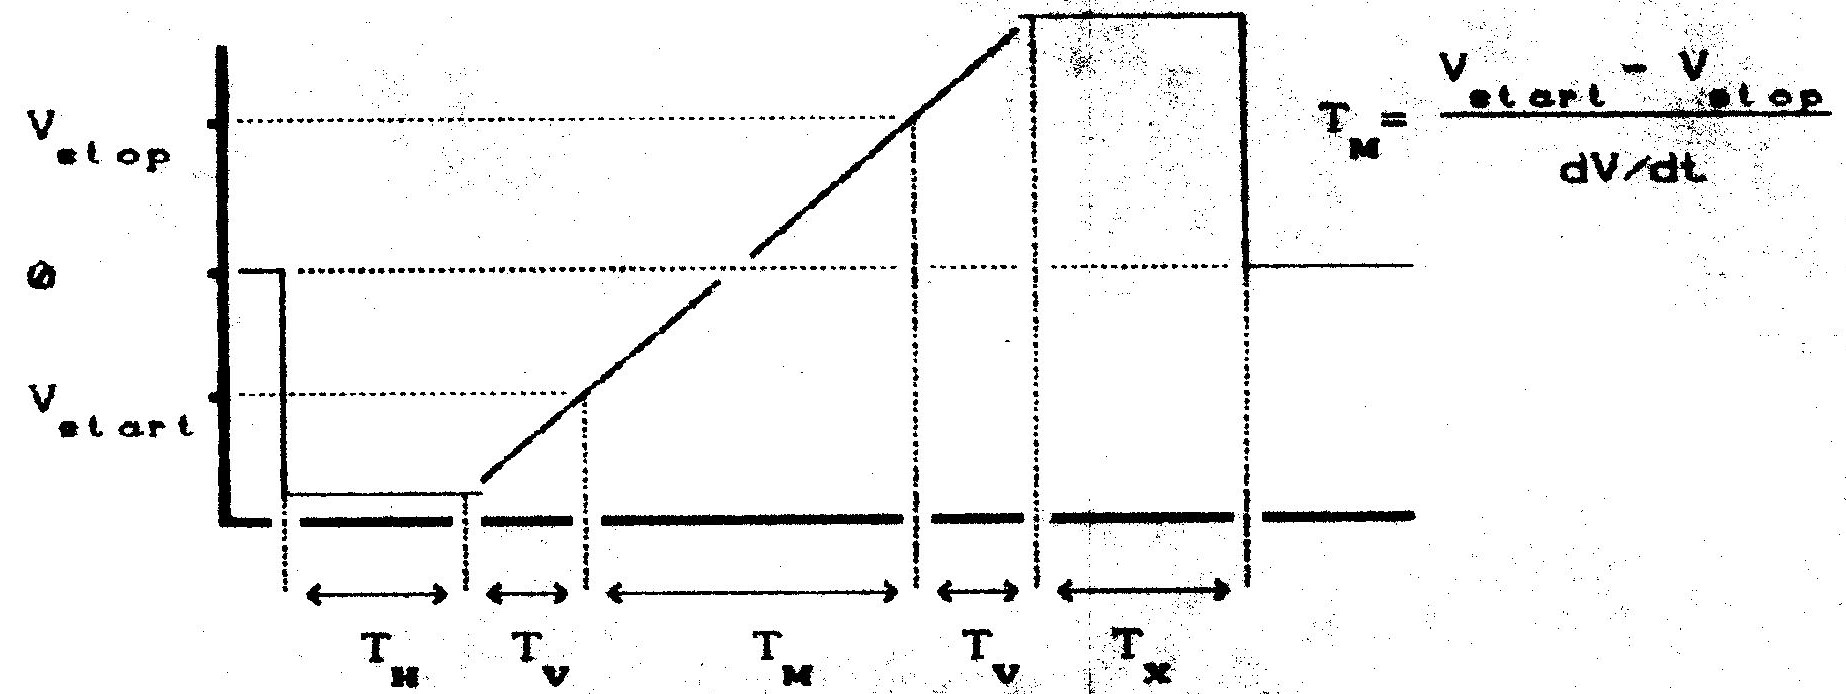
\includegraphics{Figures/fig-5-5.eps}
  \caption[Časový diagram kvázistatickej C-V metódy]{Časový diagram
    kvázistatickej C-V metódy.}\label{fig:5.5}
\end{figure}

\begin{table}[h!]\centering
  \begin{tabular}{ l p{0.5\linewidth} l l }
    parameter   & popis parametra & min. & max.hodnota\\
    \hline
    $T_H$       & čas ustálenia \dotfill & $0 s$ & neohraničené\\
    $T_V$       & merania napätia hradla a času \dotfill & $5 s$\\
    $T_M$       & merania prúdu a času \dotfill & neohraničené\\
    $T_X$       & predspracovanie dát,\\
                & uloženie dát do súboru,\\
                & posuv stolíka na ďalšiu štruktúru \dotfill & $\sim 15s$\\
    $V_{start}$ & \dotfill & $-20.0$ & $+20.0 V$\\
    $V_{stop}$  & \dotfill & $-20.0$ & $+20.0 V$\\
    $dV/dt$     & \dotfill & $\pm 0.1mV/s$ & $\pm 10.0V/s$\\
    \hline
  \end{tabular}
  \caption[Časový diagram kvázistatickej C-V metódy]{Časový diagram
    kvázistatickej C-V metódy.}\label{tab:5.3}
\end{table}

\newpage
\subsection{Metóda konštantnej šírky OPN.}\label{sec:5.4.4}

\begin{figure}[h!]\centering
  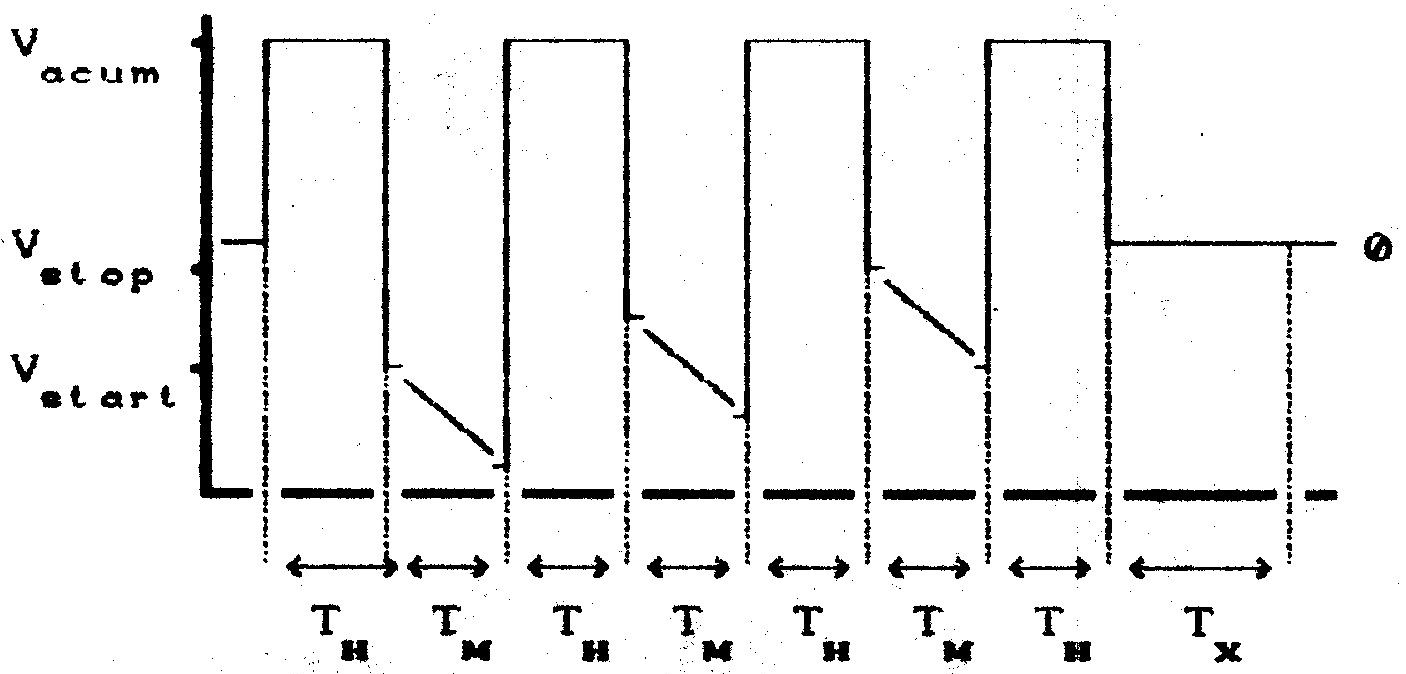
\includegraphics{Figures/fig-5-6.eps}
  \caption[Časový diagram metódy konštantnej šírky OPN]{Časový diagram
    metódy konštantnej šírky OPN}.\label{fig:5.6}
\end{figure}

\begin{table}[h!]\centering
  \begin{tabular}{ l p{0.5\linewidth} l l }
    param.      & popis parametra & min. & max.hodnota\\
    \hline
    $T_H$       & čas relaxácie minoritných nosičov náboja \dotfill & $0 s$ & neohraničené\\
    $T_M$       & čas merania, výpočet $dV/dt$ \dotfill & $10 s$ & neohraničené\\
    $T_X$       & uloženie dát do súboru,\\
                & posuv stolíka na ďalšiu štruktúru \dotfill & $\sim 2s$\\
    $V_{start}$ & \dotfill & $-40.0$ & $+40.0 V$\\
    $V_{stop}$  & \dotfill & $-40.0$ & $+40.0 V$\\
    $V_{acum}$  & \dotfill & $-40.0$ & $+40.0 V$\\
    \hline
  \end{tabular}
  \caption[Časový diagram metódy konštantnej šírky OPN]{Časový diagram
    metódy konštantnej šírky OPN.}\label{tab:5.4}
\end{table}


\begin{thebibliography}{}
\bibitem[5.1]{5.1} Mariassy P.: Riadiaca jednotka prístroja typu
  talker/listener na spojenie so zbernicou IMS\@. Diplomová práca. EF
  SVŠT Bratislava 1988.
\bibitem[5.2]{5.2} National Instruments, IEEE-488 Instrumentation
  Interface. User guide.
\bibitem[5.3]{5.3} Keithley model 642, Instruction manual.
\bibitem[5.4]{5.4} Marčuk G.I.: Metódy numerické matematiky. Academia
  Praha 1987.
\bibitem[5.5]{5.5} Cox M.G.: J. Inst. Maths. Aplics., 10 (1972) s.134.
\bibitem[5.6]{5.6} De Boor C.: J. Approx. Theory, 6 (1972) s.50.
\bibitem[5.7]{5.7} Hewlett-Packard, Operational and service manual,
  Model HP4280a.
\end{thebibliography}
